% From Juan Castaño
\documentclass[tikz,border=8mm]{standalone}
\tikzset
{
  style0/.style={thick,cyan,x={(0,1cm)},y={(1cm,0)}},
  style1/.style={thick,magenta},
  pics/arrowhead/.style={code=%定义一个新的pics style名为arrowhead箭头形状
  {
    \fill (0,0) ++ (0.15,0) --++ (-0.3,0.1) --++ (0,-0.2) -- cycle;
  }}%牛啊纯手绘
}
\begin{document}
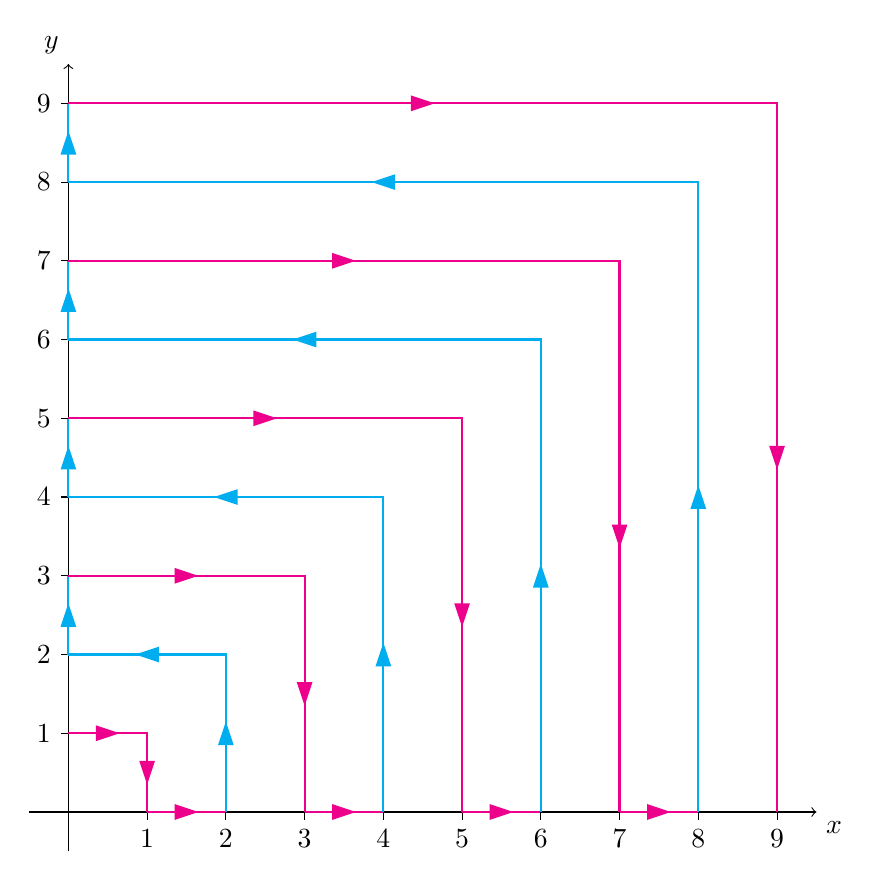
\begin{tikzpicture}
\draw[->] (-0.5,0) -- (9.5,0) node[below right] {$x$};
\draw[->] (0,-0.5) -- (0,9.5) node[above left]  {$y$};
\foreach\i in {1,...,9}
{
  \pgfmathtruncatemacro\j{mod(\i,2)}%使用math模式计算mod(\i,2)
  \draw (\i,0.1) --++ (0,-0.2) node[below] {$\i$};%绘制坐标刻度
  \draw (0.1,\i) --++ (-0.2,0) node[left]  {$\i$};
  \draw[style\j] (0,\i) -- (\i,\i) -- (\i,0);
  \pic[style\j]                  at (0.5*\i,\i) {arrowhead};
  \pic[style\j,rotate=90-180*\j] at (\i,0.5*\i) {arrowhead};
  %如果是奇数,\j=1,旋转角度为-90
  \ifnum\i<9 %特判,画最多的一段
    \draw[style\j] (\i,0) --++ (1,0);
    \pic[style\j] at (\i+0.5,0) {arrowhead};
  \fi
}
\end{tikzpicture}
\end{document}